\section{Theorie}
\subsection{Operational Amplifier in General}
The operational amplifier (=OA) is a DC-coupled difference amplifier and a general circuit is shown in
(@@).
\begin{figure}[H]
  \centering
  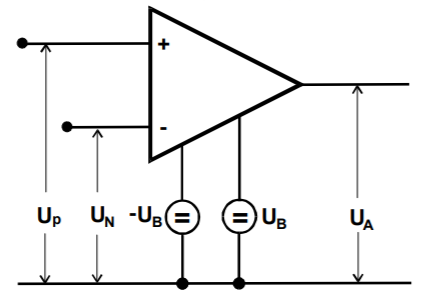
\includegraphics[scale=1]{V51Bilder/t1.png}
  \caption{General principle of an operational amplifier (operating voltages $\pm U_B$ are often left out)} \label{fig:t1} \cite{1}
\end{figure}
\noindent
With the amplification value $V$, the output voltage is
\begin{equation}
U_A = V(U_p - U_N) \label{eq:1}
\end{equation}
as long as it does not exceed the operating voltage $\pm U_B$. If it does, then $U_A = \pm U_B$ applies, depending on whether
the negative or positive value is exceeded. $V$ usually is a very large value, so minimal differences of the input voltages are enough
to exceed the operating range $\pm U_B$. Furthermore $U_A$ is in phase with the "+" - input making this the non-inverting input, and out of phase
with the "-" - input making this the inverting input.
\\
\noindent
For an ideal OA some characteristics are: infinite neutral amplification $V$ and input resistances $r_e$, and an output resistance $r_a$ of zero.
However for the real OA these values do not apply, but instead $V$ is large compared to one and depends on the frequency, $r_e$ take up large and $r_a$ small values.
For an almost-ideal OA these conditions may result only in small discrepancies on measurements compared to idealistic calculations.

\subsection{Linear Amplifier}
To get an useful operating range for the OA a negative-feedback-branch is needed, meaning that some part of $U_A$ is send back to the inverting input.
In figure (\ref{fig:lin}) a linear amplifier is shown.
\begin{figure}
  \centering
  \begin{circuitikz}
    \draw
    (0, 0) node[op amp] (opamp2) {}
    (opamp2.-) to[R,a=$R_1$] (-4, 0.5)
    (opamp2.-) (-1.5,0.49)--(-1.5,1.5)
    to[R,l=$R_N$] (1.19,1.5)
    to[short] (opamp2.out)
    (opamp2.+) --(-1.19,-1.5)
    ;
    \draw
    (0,-1.5)--(-4,-1.5)
    (0,-1.5)--(1.2,-1.5)
    ;
    \draw[<|-|>]
    (-4,-1.5)--(-4,0.49);
    \draw[<|-|>]
    (1.2,-1.5)--(opamp2.out)
    ;
    \draw[<|-|>]
    (-1.5,0.49)--(-1.5,-1.5)
    ;
    \node [right, align=left] at (-4,-0.5){$U_1$};
    \node [left, align=left] at (-1.5,-0.5){$U_N$};
    \node [right, align=left] at (1.2,-0.7){$U_A$};

  \end{circuitikz}
  \caption{Negative feedback inverting linear amplifier}
  \label{fig:lin}
\end{figure}
The negative feedback reduces the total amplification of the circuit but expands the operating range. Calculations for an ideal OA ($V = \infty = r_e$), using Kirchhoff's current law,
lead to
\begin{align}
  \frac{U_1}{R_1} + \frac{U_A}{R_N} &= 0  \label{eq:2.1}\\
  V' &= -\frac{R_N}{R_1} \label{eq:2.2} \ .
\end{align}
However, the non-idealistic characteristics will have a small influence on this equation. If the impact of a finite neutral amplification $V$ on the
amplification value $V'$ is calculated through with equation (\ref{eq:1}) and figure (\ref{lin}) a connection between $V$ and $V'$ is found
\begin{equation}
  \frac{1}{V'} \approx \frac{1}{V} + \frac{R_1}{R_N} \ . \label{eq:3}
\end{equation}
Now it becomes clear that for $V \gg \frac{R_N}{R_1}$ equations (\ref{eq:2.2}) and (\ref{eq:3}) are about the same. Concluding this, the larger the negative feedback the smaller the amplification value
and the more precisely equation (\ref{eq:2.2}) applies. Also this leads to the OA working more stable at lower amplifications.
\\
\noindent
In figure (\ref{fig:tnu}) the frequency responses between  an OA with and without negative feedback are compared to visualise the expanded bandwith by negative feedback.
\begin{figure}[H]
  \centering
  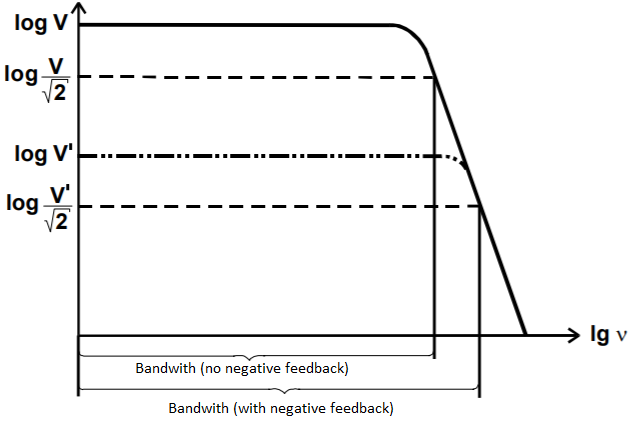
\includegraphics[scale=1]{V51Bilder/t2.png}
  \caption{Frequency response of the linear amplifier} \label{fig:tnu} \cite{1}
\end{figure}
\noindent
Furthermore the product of bandwith and $V'$ is a constant and describes the transit frequency where the amplification drops down to 1. This value is independent of the negative feedback.

\subsection{Electrometer Amplifier}
To measure high-resistance voltage sources a large input resistance $r_e$ is needed. Because that is not the case for the linear amplifier, where $r_e \approx R_1$ ($U_N \approx 0$),
the circuit is modified to the electrometer amplifier. Here the input voltage is directly connected to the non-inverting input of the OA. For the ideal OA is $r_e = \infty$ and for the real
OA $r_e \approx \SI{20}{\giga\ohm}$. \\
\noindent
\begin{figure}
  \centering
  \begin{circuitikz}
    \draw
    (0,0) node[op amp](oplol) {}
    ;
    \draw
    (-2,3)--(1.2,3)
    to[R,l=$R_1$] (1.2,1.5) to[R,l=$R_N$] (oplol.out)
    ;
    \draw (1.2,1.5)--(-1.2,1.5)--(oplol.-);
    \draw (1.2,3)--(2.8,3);
    \draw (-2,-0.5)--(oplol.+);
    \draw[<|-|>]
    (-2,-0.5)--(-2,3);
    \draw (1.5,0)--(2.8,0);
    \draw[<|-|>]
    (2.8,0)--(2.8,3);
    \node [left, align=left] at (-2, 1.75){$U_1$};
    \node [right, align=left] at (2.8, 1.5){$U_A$};
  \end{circuitikz}
  \caption{Non-inverting electrometer amplifier.}
  \label{fig:nig}
\end{figure}

\noindent
For an ideal electrometer amplifier the amplification is
\begin{equation*}
V' = \frac{R_N + R_1}{R_1}
\end{equation*}

\subsection{Inverting Integrator}
With the circuit in figure (\ref{fig:integrator}) it is possible to integrate the input voltage $U_1$.
Using Kirchhoff's law on branch point $A$, that
\begin{equation*}
\int I_C dt = C U_A
\end{equation*}
and that
\begin{equation*}
U_1 = U_0 \text{sin}\omega t
\end{equation*}
it follows for the output voltage
\begin{equation*}
U_A = \frac{U_0}{\omega R C} \text{cos}\omega t \ .
\end{equation*}
This means the output voltage is antiproportional to the frequency.
\begin{figure}[H]
  \centering
  \begin{circuitikz}
      \draw
      (0, 0) node[op amp] (opamp) {}
      (opamp.-) to[R,l=$R$] (-3, 0.5)
      (opamp.-) |- (-1, 2) to[C,a=$C$] (1, 2) -| (opamp.out)
      ;
      \draw (1.2,-1.5)--(-1.2,-1.5)--(opamp.+);
      \draw (-1,-1.5)--(-3,-1.50);
      \draw[<|-|>]
      (1.2,-1.5)--(opamp.out)
      ;
      \draw[<|-|>]
      (-3,-1.5)--(-3,0.5)
      ;
      \node [left, align=left] at (-3,-0.50){$U_1$};
      \node [right, align=left] at (1.2,-0.75){$U_A$};
      \node [above left] at (opamp.-){$A$};
  \end{circuitikz}
  \caption{Inverting integrator}
  \label{fig:integrator}
\end{figure}

\subsection{Inverting Differentiator}
With the same considerations as with the inverting integrator, for the inverting differentiator follows
the output voltage
\begin{equation*}
U_A = -\omega RCU_0 \text{cos}\omega t \
\end{equation*}
with $U_A$ being proportional to the frequency.
\begin{figure}[H]
  \centering
  \begin{circuitikz}
      \draw
      (0, 0) node[op amp] (opamp3) {}
      (opamp3.-) to[C,l=$C$] (-3, 0.5)
      (opamp3.-) |- (-1, 2) to[R,a=$R$] (1, 2) -| (opamp3.out)
      ;
      \draw (1.2,-1.5)--(-1.2,-1.5)--(opamp3.+);
      \draw (-1,-1.5)--(-3,-1.50);
      \draw[<|-|>]
      (1.2,-1.5)--(opamp3.out)
      ;
      \draw[<|-|>]
      (-3,-1.5)--(-3,0.5)
      ;
      \node [left, align=left] at (-3,-0.50){$U_1$};
      \node [right, align=left] at (1.2,-0.75){$U_A$};
  \end{circuitikz}
  \caption{Inverted differentiator}
  \label{fig:diff}
\end{figure}
\subsection{Schmitt-Trigger}
In contrast to the previous amplifiers the Schmitt-Trigger uses positive feedback. In figure (\ref{fig:schmitt}) the circuit is shown.
If a certain input voltage is reached the output voltage will jump immediately to $\pm U_B$, depending on whether the input voltage is positive or negative.
This certain voltage is adjusted by the ratio of the resistances and it follows
  \[U_A = \left\{
    \begin{array}{lr}
      + U_B & : U_1 > +\frac{R_1}{R_P}U_B \\
      - U_B & : U_1 < -\frac{R_1}{R_P}U_B
    \end{array}
  \right.
  \]
Notice that as long as $U_1$ does not exceed one of the two trigger voltages $U_A$ will stay at its current value.
The difference $2 U_B \frac{R_1}{R_P}$ between the two trigger values is called switching hysteresis.
\begin{figure}
  \centering
  \begin{circuitikz}
    \draw
    (0, 0) node[op amp] (opamp5) {}
    (opamp5.+) to[R,l=$R_1$] (-4, -0.5)
    (opamp5.+) (-1.5,-0.49)--(-1.5,-1.5)
    to[R,a=$R_p$] (1.19,-1.5)
    to[short] (opamp5.out)
    ;
    \draw
    (opamp5.-)--(-4,0.49)
    ;
    \draw[<|-|>]
    (-4,-0.49)--(-4,0.49);
    \draw[<|-|>]
    (1.2,-1.5)--(opamp2.out)
    ;
    \draw[<|-|>]
    (-1.5,0.49)--(-1.5,-0.49)
    ;
    \node [right, align=left] at (-4,0){$U_1$};
    \node [left, align=left] at (-1.5,0){$U_p$};
    \node [right, align=left] at (1.2,-0.7){$U_A$};

  \end{circuitikz}
  \caption{Schmitt-Trigger}
  \label{fig:schmitt}

\end{figure}
